

\chapter{Sequential and Concurrent VHDL}

\section{Introduction}

In this chapter we dive in more details about processes and concurrency in \verb|VHDL|.

Also we will look at new data types in \verb|VHDL|: integers and boolean.

Finally we learn how to manipulate vectors.\\

\todo{intro seq and conc}\uti{intro seq and conc:}

\begin{itemize}
\item  \textit{To re-write it later}
\end{itemize}


\newpage
\section{Processes in Depth}
\label{sec:processes_more}



As stated earlier, \verb|VHDL| program is composed from \tbi{many processes}.
In this section we dive more in depth to processes, and explore 3 different topics:

\begin{enumerate}
\item process interaction

\item process rules

\item process behavior

\end{enumerate}

Each one of these concepts is important to desing and understand a \verb|VHDL|code.

\subsection{Processes Interaction}
\label{sub:process_interact}

Processes (in plural) can interact with each other. The interaction can be:

\begin{itemize}

\item in parallel: so processes are executed simultaneously

\item sequential: exectued one after another, and usually they depend on each other

\end{itemize}

The type of interaction (execution) depends on the sensitivity list.\\


An example is shown in \autoref{fig:seq_conc_vhdl:proc_interaction}.

\begin{figure}[h]
\centering
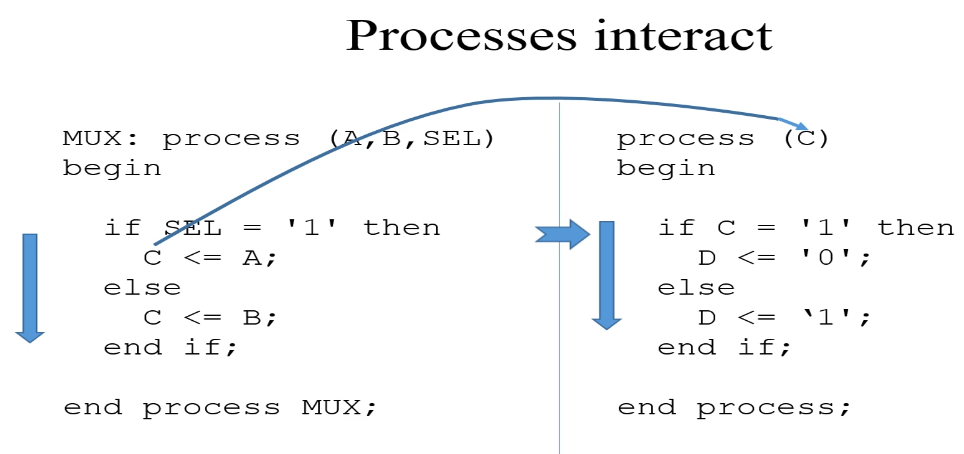
\includegraphics[scale=0.4,frame]{Figures/seq_conc_vhdl/proc_interaction}
\caption{Process interaction: sequential execution}
\label{fig:seq_conc_vhdl:proc_interaction}
\end{figure}


\begin{itemize}
\item In the $\mathrm{1}^\mathrm{st}$ process, signal \verb|C| get assigned to \verb|A| or \verb|B| depending on the value of \verb|SEL|

\item Once \verb|C| is assigned, then the $\mathrm{2}^\mathrm{nd}$ process get executed, and signal \verb|D| get assigned

\end{itemize}

\newpage
We can think that a \verb|VHDL| program consist of many processes interacting with each other, as shown in \autoref{fig:seq_conc_vhdl:process_interaction}. 

\begin{figure}[h]
\centering
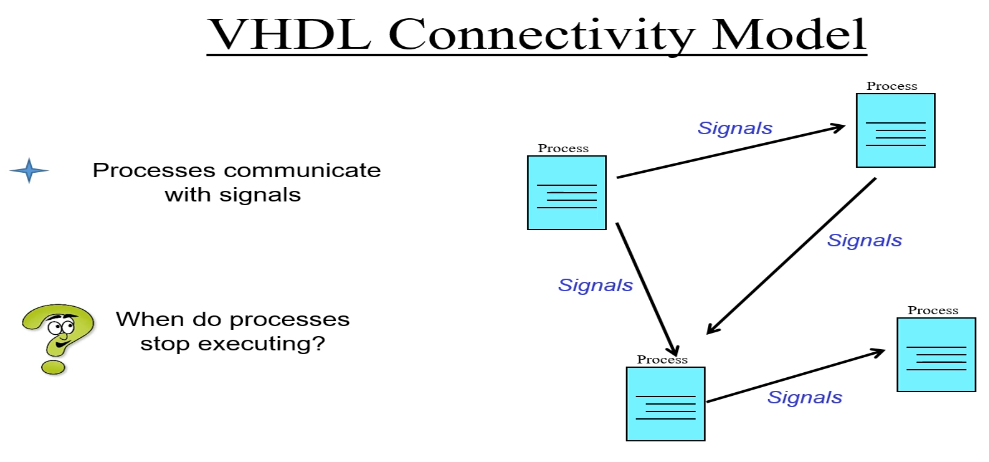
\includegraphics[scale=0.4,frame]{Figures/seq_conc_vhdl/process_interaction}
\caption{General view for process interaction}
\label{fig:seq_conc_vhdl:process_interaction}
\end{figure}

Processes interacting with each other via signal (variables) assignment.
The variables presented in process \verb|A| are in the sensitivity list of process \verb|B|

\subsection{Warning: Asynchronous Feedback}

Now we take an example shown in \autoref{fig:seq_conc_vhdl:async_feedback}, wich can cause some problems.

\begin{figure}[h]
\centering
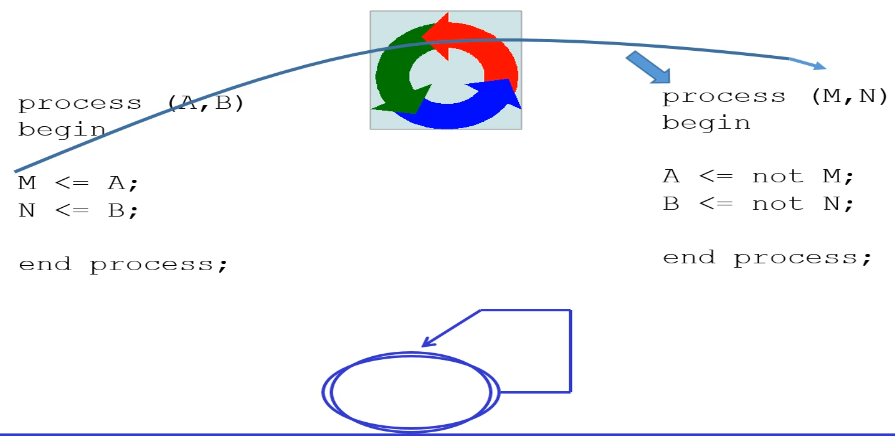
\includegraphics[scale=0.4,frame]{Figures/seq_conc_vhdl/async_feedback}
\caption{Asynchronous dilemma}
\label{fig:seq_conc_vhdl:async_feedback}
\end{figure}

\begin{itemize}

\item $\mathrm{1}^\mathrm{st}$ process (sensitive to \verb|A| and \verb|B|): we have assignment of \verb|M| and \verb|N|

\item $\mathrm{2}^\mathrm{nd}$ process we have signal assignment of \verb|A| and \verb|B|

	\begin{itemize}
	\item This cause the execution of the $\mathrm{1}^\mathrm{st}$ process because it is sensitiv to  \verb|A| and \verb|B|
	\end{itemize}

\end{itemize}

This type of signal assignment cause a loop, and will result in failur in simulation. We should be aware of such assignment and try to avoid them.

\newpage
\subsection{Process Rules}
\label{sub:process_rules}

Now let's review rules of process.

\begin{enumerate}

\item Sensitivity list

\begin{figure}[h]
\centering
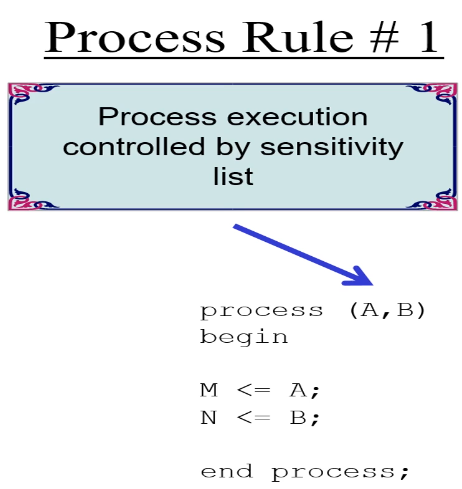
\includegraphics[scale=0.4,frame]{Figures/seq_conc_vhdl/rule_sensitivity_list}
\caption{Rule 1: Sensitivity list}
\label{fig:seq_conc_vhdl:rule_sensitivity_list}
\end{figure}


	\begin{itemize}
	\item A \verb|process| get executed if 1 or all the inputs on the sensitivity list change
	
	\item That's why we need to \tbi{include all the inputs in the sensitivity list}, so the process get exectuted correctly whenver an input change
	\end{itemize}

\item Signal assignment

\begin{figure}[h]
\centering
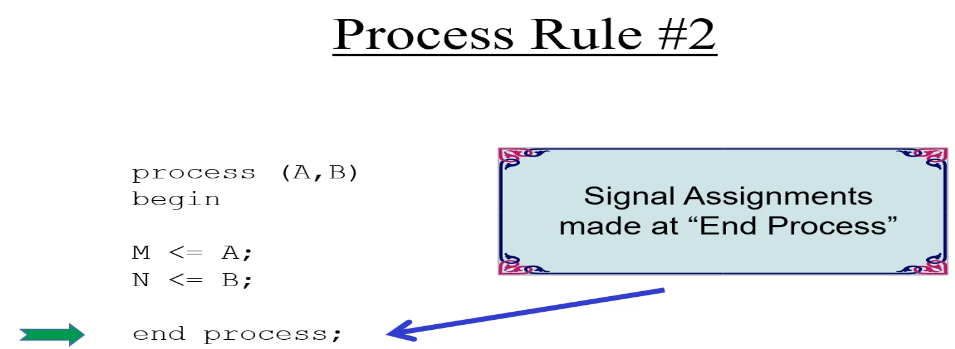
\includegraphics[scale=0.4,frame]{Figures/seq_conc_vhdl/rule_sig_assign}
\caption{Rule 2: signal assignment}
\label{fig:seq_conc_vhdl:rule_sig_assign}
\end{figure}

	\begin{itemize}
	\item This is the strangest one: signal are begin assigned \tbi{only at the end of a process}
	
	\item So at the line of execution where \verb|M<=A|, \verb|M| won't be assigned till the end of the \verb|process|
	
	\item This mean we won't be able to use \verb|M| for some intermediate computation
	
	\item We see later if we want to do such computation, we use \tbi{variables}. We will lear about them later
	\end{itemize}



\newpage
\item Multiple assignment

\begin{figure}[h]
\centering
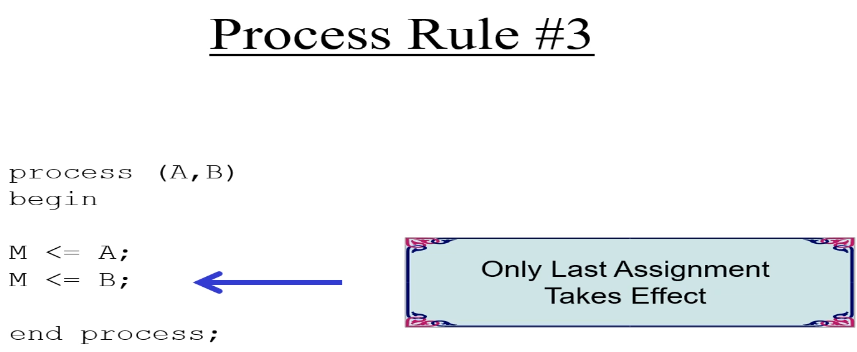
\includegraphics[scale=0.4,frame]{Figures/seq_conc_vhdl/rule_multip_assign}
\caption{Rule 3: Multiple assignment}
\label{fig:seq_conc_vhdl:rule_multip_assign}
\end{figure}

	\begin{itemize}
	\item If we make multiple assignment to \tbi{same signal}, only the last one get executed
	
	\item So \verb|M <= A;| get ignored
	
	\item And \verb|M <= B;| get executed at the \tbi{end} of process (recall rule 2)
	\end{itemize}


\end{enumerate}

\newpage
\subsection{Process Behavior}

Now we learned process rules in \ref{sub:process_rules}, let's take an example about the execution of a process, shown in \autoref{fig:seq_conc_vhdl:process_behavior_ques}.

\begin{figure}[h]
\centering
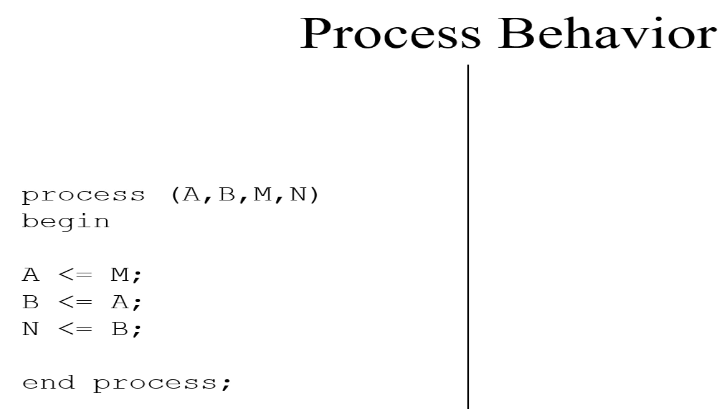
\includegraphics[scale=0.4,frame]{Figures/seq_conc_vhdl/process_behavior_ques}
\caption{Process Behavior}
\label{fig:seq_conc_vhdl:process_behavior_ques}
\end{figure}

\underline{Question:} what are the final values of \verb|A|,\verb|B| and \verb|N|, if this process is executed for 3 times ?\\

\underline{Answer:} values are shown in \autoref{fig:seq_conc_vhdl:process_behavior_ans}.

\begin{figure}[h]
\centering
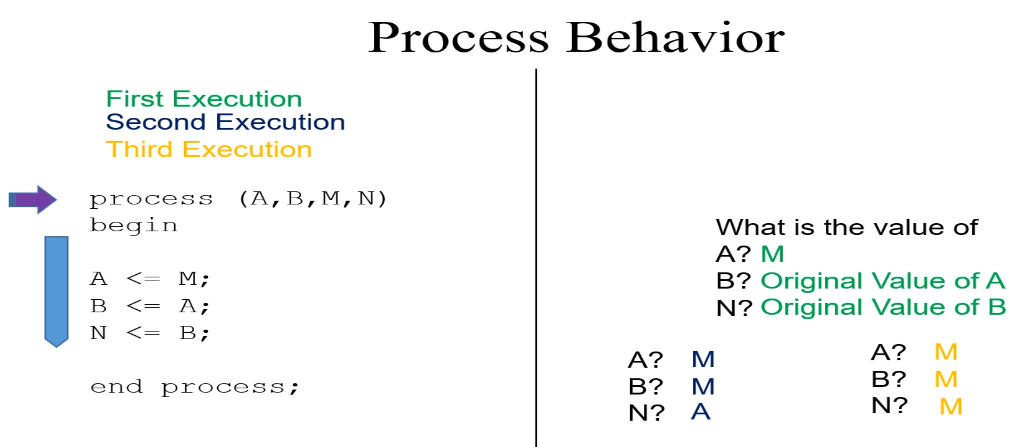
\includegraphics[scale=0.4,frame]{Figures/seq_conc_vhdl/process_behavior_ans}
\caption{Process Behavior}
\label{fig:seq_conc_vhdl:process_behavior_ans}
\end{figure}


\newpage
\section{Data Types: Integer and Boolean}

So far we dealt with bit and bit vectors data types (\ref{sub:vectors}), we continue explore other data types in \verb|VHDL| such as integers and boolean in this section.\\

An example is shown in \autoref{fig:seq_conc_vhdl:int_data_type}.

\begin{figure}[h]
\centering
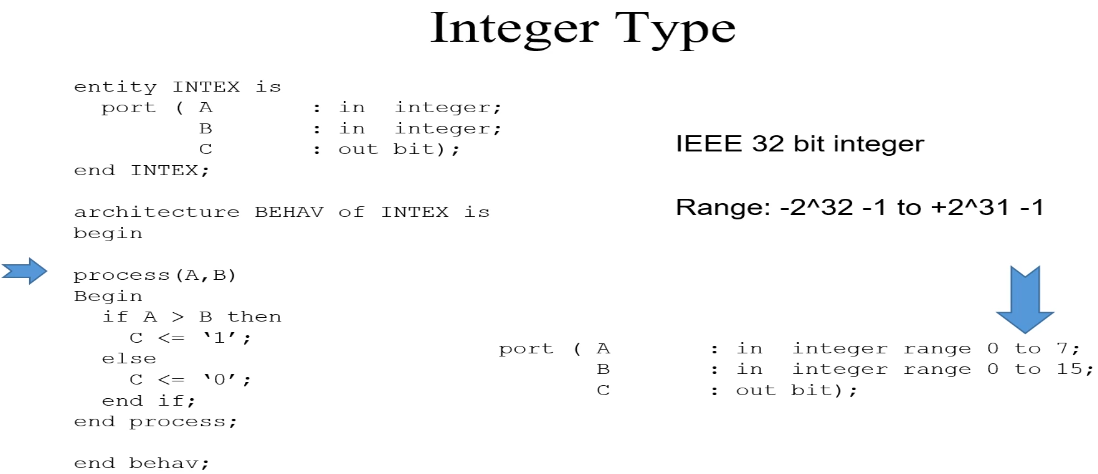
\includegraphics[scale=0.4,frame]{Figures/seq_conc_vhdl/int_data_type}
\caption{Integer data type in VHDL}
\label{fig:seq_conc_vhdl:int_data_type}
\end{figure}

\begin{itemize}

\item In \verb|VHDL|, and since almost we don't need huge range of values of integers in our application, we can specify the range of intergers we need as shown at the right bottom of \autoref{fig:seq_conc_vhdl:int_data_type}

\end{itemize}

Also \verb|VHDL| support boolean as shown in \autoref{fig:seq_conc_vhdl:bool_data_type}.

\begin{figure}[h]
\centering
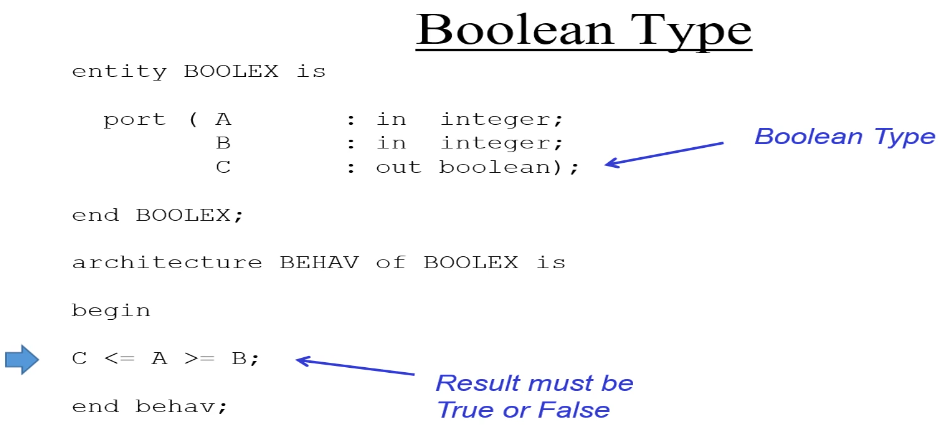
\includegraphics[scale=0.4,frame]{Figures/seq_conc_vhdl/bool_data_type}
\caption{Boolean data type in VHDL}
\label{fig:seq_conc_vhdl:bool_data_type}
\end{figure}

\begin{itemize}

\item In the example, \verb|C| get assigned to 0 or 1 whether the condition \verb|A >= B| is true or not

\end{itemize}

\newpage
\section{Summary Processes}

Processes (\ref{sec:processes_more}):

\begin{itemize}

\item $\mathrm{1}^\mathrm{st}$ recall definition from \autoref{chap:intro_vhdl}:

	\begin{itemize}
	\item processe include the code which execute \tbi{sequentially}
	
	\item should contain a sensitivity list $\leftrightarrow$ \verb|process(A,B)| $\leftrightarrow$ all inputs should be mentioned in the sensitivity list
	\end{itemize}

\item Type of interaction (\ref{sub:process_interact}): 

	\begin{itemize}
	\item concurrent or sequential
	
		\begin{itemize}
		\item recall from \autoref{chap:intro_vhdl}, that when we work with concurrancy, order of execution is not important since all of them will be executed in parallel using FPGA hardware capability
		\end{itemize}
	
	\item Depending on the sensistivity list (see \autoref{fig:seq_conc_vhdl:proc_interaction})
	\end{itemize}


\item Process rules (\ref{sub:process_rules})

	\begin{itemize}
	\item sensitivity list should contains all the input
	
	\item assignment happens at the end of the process
	
	\item if multiple assignment to same signal, only the last one get executed
	\end{itemize}


\end{itemize}








